\subsection{表面元素}

本节中，令 q 表示包含于 A 的根基中的一个理想，并令 M 为非零有限生成 A-模，使得 M/qM 具有有限长度。

命题 8. --- 令 \(\delta > 0\) 为一个整数，\(x\) 为 \(\mathfrak{q}^{\delta}\) 中的元素，\(\xi\) 为它在 \(\mathrm{gr}_{\delta}(\mathbf{A}) = \mathfrak{q}^{\delta}/\mathfrak{q}^{\delta+1}\) 中的类，并令 \(\varphi\) 表示 \(\xi\) 在 \(\mathrm{gr}(\mathbf{A})\)-模 \(\mathrm{gr}(\mathbf{M})\) 上的乘法作用。

\begin{enumerate}
\def\labelenumi{\alph{enumi})}
\item
  A-模 M/xM 的维数等于 \(\dim_{\mathbf{A}}(\mathbf{M})\) 或 \(\dim_{\mathbf{A}}(\mathbf{M}) - 1\)。在第二种情形下，有 \(e_{\mathfrak{q}}(\mathbf{M}/x\mathbf{M}) \geqslant \delta e_{\mathfrak{q}}(\mathbf{M})\)。
\item
  假设 \(\dim_{\mathbf{A}}(\mathbf{M}) \geqslant 1\)，并且 \(\varphi\) 的核作为 A/q-模具有有限长度。则有 \(\dim_{\mathbf{A}}(\mathbf{M}/x\mathbf{M}) = \dim_{\mathbf{A}}(\mathbf{M}) - 1\)。此外：
\end{enumerate}

\begin{enumerate}
\def\labelenumi{(\roman{enumi})}
\item
  若 \(\dim_{\mathbf{A}}(\mathbf{M}) > 1\)，则有 \(e_{\mathfrak{q}}(\mathbf{M} / x\mathbf{M}) = \delta e_{\mathfrak{q}}(\mathbf{M})\)。
\item
  若 \(\dim_{\mathbf{A}}(\mathbf{M}) = 1\)，则对每个整数 \(n \geqslant 0\)，有
\end{enumerate}

\[
n \delta e _ {\mathfrak {q}} (\mathrm{M}) \leqslant \operatorname{long} _ {\mathrm{A}} (\mathrm{M} / x ^ {n} \mathrm{M}) \leqslant n \delta e _ {\mathfrak {q}} (\mathrm{M}) + \operatorname{long} _ {\mathrm{A} / \mathfrak {q}} (\operatorname{Ker} \varphi^ {n}),
\]

其中 \(\varphi^n\) 是第 \(n\) 次自同态 \(\varphi\) 的迭代，并且

\[
\delta e _ {\mathfrak {q}} (\mathbf {M}) = e _ {x \mathbf {A}} (\mathbf {M}) \leqslant \operatorname{long} _ {\mathbf {A}} (\mathbf {M} / x \mathbf {M}).
\]

置 \(\mathbf{M}'' = \mathbf{M} / x\mathbf{M}\)；考察 Hilbert-Samuel 级数 \(\mathbf{H}_{\mathbf{M}} = \mathbf{H}_{\mathbf{M},\mathfrak{q}}\) 和 \(\mathbf{H}_{\mathbf{M}''} = \mathbf{H}_{\mathbf{M}'',\mathfrak{q}}\)，以及 Poincaré 级数 \(\mathbf{P}(\mathbf{T}) = \sum_{n\geqslant 0}\mathrm{long}_{\mathbf{A} / \mathfrak{q}}(\mathrm{Ker}\varphi_n)\mathbf{T}^n\)。根据第 4 节第 3 号定理 2 和第 4 号备注 2，有

\[
\mathrm{H} _ {\mathbf {M}} (\mathrm{T}) = (1 - \mathrm{T}) ^ {- d} \mathrm{R} _ {\mathbf {M}} (\mathrm{T}), \quad \mathrm{H} _ {\mathbf {M} ^ {\prime \prime}} (\mathrm{T}) = (1 - \mathrm{T}) ^ {- d ^ {\prime \prime}} \mathrm{R} _ {\mathbf {M} ^ {\prime \prime}} (\mathrm{T}),
\]

其中 \(d = \dim_{\mathbf{A}}(\mathbf{M})\)，\(d'' = \dim_{\mathbf{A}}(\mathbf{M}'')\)，\(\mathbf{R}_{\mathbf{M}}\) 和 \(\mathbf{R}_{\mathbf{M}''}\) 属于 \(\mathbf{Z}[T]\)，\(\mathbf{R}_{\mathbf{M}}(1) = e_{\mathfrak{q}}(\mathbf{M})\)，\(\mathbf{R}_{\mathbf{M}''}(1) = e_{\mathfrak{q}}(\mathbf{M}'')\)。由第 4 节第 5 号引理 6，在 \(\mathbf{Z}((T))\) 中有不等式

\[
\left(1 - \mathrm{T} ^ {\delta}\right) \mathrm{H} _ {\mathbf {M}} ^ {(1)} \leqslant \mathrm{H} _ {\mathbf {M} ^ {\prime \prime}} ^ {(1)} \leqslant \left(1 - \mathrm{T} ^ {\delta}\right) \mathrm{H} _ {\mathbf {M}} ^ {(1)} + \mathrm{T} ^ {\delta} \mathrm{P} ^ {(1)}.
\]

令 \(\mathrm{R}(\mathrm{T}) = (1 - \mathrm{T}^{\delta}) / (1 - \mathrm{T}) = 1 + \mathrm{T} + \cdots + \mathrm{T}^{\delta-1},\) 此式也可写成

\[
\begin{array}{r l} (1) & (1 - \mathrm{T}) ^ {- d} \mathrm{R(T)} \mathrm {R_ {M} (T)} \leqslant (1 - \mathrm{T}) ^ {- d ^ {\prime \prime} - 1} \mathrm {R_ {M^ {\prime\prime}} (T)} \leqslant \\ & \leqslant (1 - \mathrm{T}) ^ {- d} \mathrm{R(T)} \mathrm {R_ {M} (T)} + (1 - \mathrm{T}) ^ {- 1} \symrm {T^ {\delta} P(T)}. \end{array}
\]

由第 4 节第 1 号引理 2，第一条不等式 (1) 蕴含：要么 \(d'' \geqslant d\)，要么 \(d'' = d - 1\) 且 R(1) R \(_{M}\) (1) \(\leqslant\) R \(_{M''}\) (1)，即 \(\delta e_{\mathfrak{q}}(\mathbf{M}) \leqslant e_{\mathfrak{q}}(\mathbf{M}'')\)。这证明了 \(a\) )，因为 \(d'' \leqslant d\)。

在 \(b\) ) 的假设下，有 \(\mathbf{P}(\mathbf{T}) \in \mathbf{Z}[\mathbf{T}]\) 且 \(\mathbf{P}(1) = \text{long}_{\mathbf{A}}(\text{Ker } \varphi)\)。第二个不等式 (1) 写作

\[
(1 - \mathrm{T}) ^ {- d ^ {\prime \prime} - 1} \mathrm{R} _ {\mathrm{M} ^ {\prime \prime}} (\mathrm{T}) \leqslant (1 - \mathrm{T}) ^ {- d} \left(\mathrm{R} (\mathrm{T}) \mathrm{R} _ {\mathrm{M}} (\mathrm{T}) + \mathrm{T} ^ {\delta} (1 - \mathrm{T}) ^ {d - 1} \mathrm{P} (\mathrm{T})\right).
\]

设 \(d > 1\)；则第 4 节第 1 号引理 2 蕴含 \(d'' + 1 \leqslant d\)，因而 \(d'' = d - 1\)，这是根据证明中的 \(a\) ) 部分得到的；于是有

\[
\mathrm{R} _ {\mathbf {M} ^ {\prime \prime}} (1) \leqslant \mathrm{R} (1)\cdot \mathrm{R} _ {\mathbf {M}} (1)
\]

(同上)，从而得到 (i)。

现在设 \(d=1\)。由同上，有 \(d''=0\)，并且

\[
\mathrm{R} _ {\mathbf {M} ^ {\prime \prime}} (1) \leqslant \mathrm{R} (1)\cdot \mathrm{R} _ {\mathbf {M}} (1) + \mathrm{P} (1).
\]

因此，\(\mathbf{M}''\) 具有有限长度，且其长度等于 \(e_{\mathfrak{q}}(\mathbf{M}^{\prime \prime}) = \mathbf{R}_{\mathbf{M}''}(1)\)，从而得到

\[
\delta e _ {\mathfrak {q}} (\mathrm{M}) \leqslant \operatorname{long} _ {\mathrm{A}} (\mathrm{M} / x \mathrm{M}) \leqslant \delta e _ {\mathfrak {q}} (\mathrm{M}) + \operatorname{long} _ {\mathrm{A}} (\operatorname{Ker} \varphi).\tag{2}
\]

令 \(n \geqslant 1\) 为一个整数。在 (2) 中将 \(x\) 替换为 \(x^n\)；于是有

\[
n \delta e _ {\mathfrak{q}} (\mathbf {M}) \leqslant \operatorname{long} _ {\mathbf {A}} (\mathbf {M} / x ^ {n} \mathbf {M}) \leqslant n \delta e _ {\mathfrak{q}} (\mathbf {M}) + \operatorname{long} _ {\mathbf {A}} (\operatorname{Ker} \varphi^ {n}).\tag{3}
\]

显然，诺特 gr(A)-模 gr(M) 的子模 Ker \(\varphi^{n}\) 构成递增序列，因而最终稳定，并且每个子模作为 A/q-模都具有有限长度。将不等式 (3) 除以 \(n \geqslant 1\)，并令 \(n\) 趋于 \(+\infty\)，从而得到 \(e_{xA}(M) = \delta e_{\mathfrak{q}}(\mathbf{M})\)，这是 \(e_{xA}(M)\) 的定义。

引理 3. — 令 R 为次数 ≥ 0 的分次诺特环，E 为有限生成分次 R-模，并满足 \(E_{n}\) 是有限长度的 \(R_{0}\)-模，且这一点对每个 \(n \in Z\) 都成立。以下条件等价：

\begin{enumerate}
\def\labelenumi{(\roman{enumi})}
\item
  E 是具有有限长度的 R-模；
\item
   存在整数 \(n_0\)，使得 \(\mathrm{E}_n = 0\) 对所有 \(n \geqslant n_0\) 都成立；
\item
  \(\mathbf{R}\) 的每个与 \(\mathbf{E}\) 相关的素理想都包含 \(\mathbf{R}_{+} = \bigoplus_{n\geqslant 1}\mathbf{R}_{n}\)。
\item
  \((i) \Leftrightarrow (ii)\)：这是显然的。
\item
  \((iii) \Rightarrow (i)\)：令 \(p\) 为一个与 E 相关的素理想。若满足 (iii)，则有 \(p = p_0 + R_+\)，其中 \(p_0\) 是 \(R_0\) 的素理想，且 R-模 \(R/p\) 同构于 \(R_0/p_0\)。根据 IV, § 3, n° 1, 命题 1 的推论，\(R_0\)-模 \(R_0/p_0\) 同构于某个 \(E_k\) 的子模，因而具有有限长度。因此 R/p 具有有限长度。根据 IV, § 2, n° 5, 命题 7，p 因而是极大理想。由于 p 任意，R-模 E 具有有限长度（同上）。
\item
  \((i) \Rightarrow (iii)\)：令 \(p\) 为一个与 E 相关的素理想。则 \(p\) 是分次的（IV, § 3, 第 1 号, 命题 1）且是极大的（IV, § 2, 第 5 号, 命题 7），因而包含 \(R_{+}\)（§ 6, 第 2 号, 引理 1）。
\end{enumerate}

命题 9. --- 记 \(\mathfrak{p}_1, \ldots, \mathfrak{p}_r\) 为分次环 \(\mathrm{gr}(\mathrm{A}) = \bigoplus_{n} (\mathfrak{q}^n / \mathfrak{q}^{n+1})\) 的素理想中那些与分次模 \(\mathrm{gr}(\mathrm{M}) = \bigoplus_{n} (\mathfrak{q}^n \mathrm{M} / \mathfrak{q}^{n+1} \mathrm{M})\) 相关且不包含 \(\mathrm{gr}_1(\mathrm{A}) = \mathfrak{q} / \mathfrak{q}^2\) 的素理想。令 \(\delta\) 为整数 \(>0\)，\(\xi\) 为 \(\mathrm{gr}_{\delta}(\mathrm{A})\) 中的元素，并令 \(\varphi : \mathrm{gr}(\mathrm{M}) \to \mathrm{gr}(\mathrm{M})\) 表示比值为 \(\xi\) 的 \(\mathrm{gr}(\mathrm{M})\) 上的伸缩。映射 \(\varphi_n\) 对所有充分大的 \(n\) 都是单射，当且仅当 \(\xi^n\) 不属于任何 \(\mathfrak{p}_i\)。

事实上，gr(A)-模 Ker φ 的相关素理想正是 gr(M) 的相关素理想中包含 ξ 的那些（IV, § 1, 第 1 号, 定义 1）。根据引理 3，(Ker φ) \(_n\) 在 \(n\) 足够大时为零，当且仅当这些理想都包含 \(\mathrm{gr}_{+}(\mathrm{A})\)（或等价地，包含 \(\mathrm{gr}_{1}(\mathrm{A})\)），命题得证。

定义 2. --- 令 A 为诺特环，q 为包含于 A 的根基中的 A-理想，并令 M 为有限生成 A-模，使得 M/qM 具有有限长度。如果 x 属于 q，且对所有充分大的 n，由 x 的乘法所诱导的映射 \(\mathfrak{q}^{n}\mathbf{M}/\mathfrak{q}^{n+1}\mathbf{M} \to \mathfrak{q}^{n+1}\mathbf{M}/\mathfrak{q}^{n+2}\mathbf{M}\) 是单射，则称 A 的元素 x 关于 q 对 M 是表面元素。

备注。--- 1) 令 δ 为一个 \textgreater{} 0 的整数。若 \(x \in \mathfrak{q}^{\delta}\)，且对所有充分大的 n，由 x 的乘法所诱导的映射 \(\mathfrak{q}^{n}\mathbf{M}/\mathfrak{q}^{n+1}\mathbf{M} \to \mathfrak{q}^{n+\delta}\mathbf{M}/\mathfrak{q}^{n+\delta+1}\mathbf{M}\) 是单射，有时称 A 的元素 x 关于 q 对 M 是阶数为 δ 的表面元素。按此术语，定义 2 意义下的表面元素就是阶数为 1 的表面元素。

\begin{enumerate}
\def\labelenumi{\arabic{enumi})}
\setcounter{enumi}{1}
\item
   采用命题 9 的记号，\(x\) 是阶数为 \(\delta\) 的表面元素，当且仅当它的类 \(\xi\) 在 \(\mathrm{gr}_{\delta}(\mathbf{A})\) 中不属于任何一个 \(\mathfrak{p}_i\)。
\item
  根据 III, § 1, 第 4 号, 命题 8，存在一个 \(\mathrm{gr}(\mathrm{A})\) 中次数为 \(>0\) 且不属于任何一个 \(\mathfrak{p}_i\) 的齐次元素。因此，存在整数 \(\delta > 0\) 以及一个对 M 阶数为 \(\delta\) 的表面元素。
\item
   假设 A 是局部环，剩余域为 \(k\)，并考察典范满射 \(\lambda: \mathfrak{q} \to \mathfrak{q} \otimes_{\mathbf{A}} k\)。它是典范映射 \(\mathfrak{q} \to \mathfrak{q}/\mathfrak{q}^2\) 与 \(\overline{\lambda}: \mathfrak{q}/\mathfrak{q}^2 \to \mathfrak{q} \otimes_{\mathbf{A}} k\) 的复合。根据 Nakayama 引理，\(V_i = \overline{\lambda}(\mathfrak{p}_i \cap (\mathfrak{q}/\mathfrak{q}^2))\) 是 \(\mathfrak{q} \otimes_{\mathbf{A}} k\) 的向量子空间，且上述各空间都不等于 \(\mathfrak{q} \otimes_{\mathbf{A}} k\)；若 \(\alpha \in \mathfrak{q} \otimes_{\mathbf{A}} k\) 不属于任何一个 \(V_i\)，则 \(\lambda^{-1}(\alpha)\) 中的元素都是对 M 的表面元素（命题 9）。若 \(k\) 是无限域，则 \(V_i\) 的并集不等于 \(\mathfrak{q} \otimes_{\mathbf{A}} k\)，因而存在对 M 的表面元素。
\end{enumerate}

定理 1. --- 令 A 为诺特环，q 为包含于 A 的根基中的 A-理想，并令 M 为有限生成 A-模，使得 M/qM 具有有限长度。令 \(x_{1}, \ldots, x_{m}\) 为 q 中元素的有限序列。置 \(x = Ax_{1} + \cdots + Ax_{m} \subset q\)。

\begin{enumerate}
\def\labelenumi{\alph{enumi})}
\item
  有 \(\dim_{\mathbf{A}}(\mathbf{M} / \mathfrak{x}\mathbf{M})\geqslant \dim_{\mathbf{A}}(\mathbf{M}) - m.\)
\item
  若 \(\dim_{\mathbf{A}}(\mathbf{M} / \mathfrak{x}\mathbf{M}) = \dim_{\mathbf{A}}(\mathbf{M}) - m\)，则 \(e_{\mathfrak{q}}(\mathbf{M} / \mathfrak{x}\mathbf{M}) \geqslant e_{\mathfrak{q}}(\mathbf{M})\)。
\item
  若 \(m < \dim_{\mathbf{A}}(\mathbf{M})\)，且对于 \(i = 1, \ldots, m\)，A 的元素 \(x_{i}\) 关于 q 对 \(\mathbf{M}/(x_{1}\mathbf{M} + \cdots + x_{i-1}\mathbf{M})\) 是表面元素，则有
\end{enumerate}

\[
\dim_{\mathbf{A}}(\mathbf{M} / \mathfrak{x}\mathbf{M}) = \dim_{\mathbf{A}}(\mathbf{M}) - m \quad\text{且}\quad e_{\mathfrak{q}}(\mathbf{M} / \mathfrak{x}\mathbf{M}) = e_{\mathfrak{q}}(\mathbf{M}).
\]

\begin{enumerate}
\def\labelenumi{\alph{enumi})}
\setcounter{enumi}{3}
\tightlist
\item
  若 \(m = \dim_{\mathbf{A}}(\mathbf{M})\)，且对于 \(i = 1, \ldots, m\)，A 的元素 \(x_{i}\) 关于 q 对 \(\mathbf{M}/(x_{1}\mathbf{M} + \cdots + x_{i-1}\mathbf{M})\) 是表面元素，则有
\end{enumerate}

\[
e _ {\mathfrak {q}} (\mathbf {M}) = e _ {\mathfrak {x}} (\mathbf {M}) \leqslant \operatorname{long} (\mathbf {M} / \mathfrak{x}\mathbf{M}) <   + \infty .
\]

当 \(a\) )、\(b\) ) 和 \(c\) ) 在 \(m = 1\) 时由命题 8 得出，一般情形则由归纳法得到。假设 \(d\) ) 的假设成立，并置 \(\mathbf{x}' = \mathrm{A}x_{1} + \cdots + \mathrm{A}x_{m-1}\) 与 \(\mathbf{M}' = \mathbf{M}/\mathbf{x}'\mathbf{M}\)，从而 \(\mathbf{M}/\mathbf{x}\mathbf{M}\) 可识别为 \(\mathbf{M}'/x_{m}\mathbf{M}'\)。于是根据 \(c\) )，有 \(\dim_{\mathbf{A}}(\mathbf{M}') = 1\) 且 \(e_{\mathfrak{q}}(\mathbf{M}) = e_{\mathfrak{q}}(\mathbf{M}')\)。由命题 8，\(\mathbf{M}/\mathbf{x}\mathbf{M}\) 具有有限长度，且 \(e_{\mathfrak{q}}(\mathbf{M}') = e_{x_{m}\mathbf{A}}(\mathbf{M}') \leqslant \text{long}(\mathbf{M}/\mathbf{x}\mathbf{M})\)。但是，由于 \(x_{m}^{n}\mathbf{M}' = \mathfrak{x}^{n}\mathbf{M}'\) 对每个 \(n\) 都成立，故 \(e_{x_{m}\mathbf{A}}(\mathbf{M}') = e_{\mathfrak{x}}(\mathbf{M}')\)。另一方面，有 \(e_{\mathfrak{x}}(\mathbf{M}') \geqslant e_{\mathfrak{x}}(\mathbf{M})\)；这是由 \(b\) ) 得出的，其中将 \(m\) 替换为 \(m - 1\)，将 \(x\) 替换为 \(x'\)，并将 \(q\) 替换为 \(\mathfrak{x}\)。因此，有

\[
e _ {\mathfrak {x}} (\mathrm{M}) \leqslant e _ {\mathfrak {x}} (\mathrm{M} ^ {\prime}) = e _ {x _ {m} \mathrm{A}} (\mathrm{M} ^ {\prime}) = e _ {\mathfrak {q}} (\mathrm{M} ^ {\prime}) = e _ {\mathfrak {q}} (\mathrm{M}).
\]

由于 \(\mathfrak{x}\) 包含于 \(\mathfrak{q}\)，这意味着 \(e_{\mathfrak{x}}(\mathbf{M}) = e_{\mathfrak{q}}(\mathbf{M})\)（第 1 号, 备注 1），证明完成。

推论。--- 假设 A 是局部环且剩余域无限，并令 \(d = \dim_{\mathbf{A}}(\mathbf{M})\)。存在 q 中元素的序列 \(x_{1}, \ldots, x_{d}\)，使得置 \(x = Ax_{1} + \cdots + Ax_{d}\) 后，有

\[
e _ {\mathfrak {q}} (\mathbf {M}) = e _ {\mathfrak {x}} (\mathbf {M}) \leqslant \operatorname{long} (\mathbf {M} / \mathfrak{x}\mathbf{M}) <   + \infty .
\]

这立即由定理和备注 4 得出。

备注 5. --- 在前述推论的情形下，有

\[
e _ {\mathfrak {q}} (\mathrm{M}) = e _ {\mathfrak {x}} (\mathrm{M}) \leqslant \operatorname{long} (\mathrm{M} / \mathfrak {x} \mathrm{M})
\]

\pandocbounded{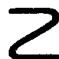
\includegraphics[keepaspectratio]{images/part001_8adf5445.jpg}}

并且 \(\operatorname{long}(\mathbf{M} / \mathfrak{q}\mathbf{M})\leqslant \operatorname{long}(\mathbf{M} / \mathfrak{x}\mathbf{M})\)；以下三种情形

\[
e _ {\mathfrak {q}} (\mathrm{M}) <   \operatorname{long} (\mathrm{M} / \mathfrak {q} \mathrm{M}), e _ {\mathfrak {q}} (\mathrm{M}) = \operatorname{long} (\mathrm{M} / \mathfrak {q} \mathrm{M}), e _ {\mathfrak {q}} (\mathrm{M}) > \operatorname{long} (\mathrm{M} / \mathfrak {q} \mathrm{M})
\]

是可能的（第~106页，习题 16 和 17）。

